\chapter{Mathematical Analysis}

\section{Moment of Inertia Calculation}

The method of moment of inertia ($I$) calculation that we chosed is the disk method. This method involves summing up the contributions of many small disk elements, each with its own moment of inertia. 

\bigbreak{}

For a cylindrical cup, the most appropriate integration method to calculate the moment of inertia is the disk method. The disk method is well-suited for rotationally symmetric objects like cylinders.

\bigbreak{}

The general formula for the moment of inertia for a differential mass element $\partial{m}$ at a distance $r$ from the axis of rotation is given by:

\[I = \int\limits_a^b r^2 \partial{m}\]

\noindent where $a$ and $b$ represent the limits of integration along the radial direction.

In this context, $r$ is the distance of a differential mass element from the axis of rotation. Since our object is symmetric, $r$ can be expressed as 

\[ r = f(x) - g(x)\]

The differential mass $\partial{m}$ is expressed as $\partial{m} = \sigma \partial{A}$, where $\sigma$ is the mass per unit area and $\partial{A}$ is the area of the differential element.

\bigbreak{}

Putting it all together, the moment of inertia can be computed as follows:

\[ I = \int\limits_{a}^{b} {\left(f(x) - g(x)\right)}^2\sigma\partial{A} \]

\newpage
\thispagestyle{plain}

Given that $\partial{A}$ is a thin annular ring with thickness $\partial{x}$, the area of the ring is $\partial{A} = 2\pi x\partial{x}$ (circumference $\times$ thickness). Therefore, the moment of inertia equation becomes:

\[ I = \int\limits_{a}^{b} 2\pi x {(f(x) - g(x))}^2\sigma\partial{x} \]

\begin{center}
    \begin{figure}
        \centering
        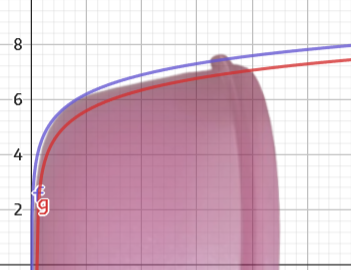
\includegraphics[width=0.4\textwidth]{assets/graph.png}
        \caption{Graph of $f(x)$ and $g(x)$}       
    \end{figure}
\end{center}

\begin{align*}
    f(x) &= \ln(x) + 5.5 \\
    g(x) &= \ln(x - 0.2)  + 5 \\
    I &= \int\limits_{1}^{10} 2\pi x {\left(\ln\left(\frac{x}{x-0.2}\right) + 0.5\right)}^2\partial{x} \approx 90~g/cm^2 \\
    &\approx 0.09~kg/m^2
\end{align*}

\section{Torsion Modulus Calculation}

The torsion modulus ($J$) is a measure of the stiffness of the elastic wire used in the experiment. It relates the torque applied to the wire (due to the twist) to the resulting angular displacement. Using the computed moment of inertia ($I$) obtained from the last calculations, we can find $J$ by rearranging the equation for the period of oscillation ($T$):

\begin{align*}
    T &= 2\pi\sqrt{\frac{I}{J}} \\
    J &= \frac{4\pi^2I}{T^2}
\end{align*}

\newpage
\thispagestyle{plain}

\noindent Here, $T$ is the period of oscillation of the pendulum, which can be measured experimentally. By substituting the known values of $I$, $T$ and $\pi$ (let's assume $\pi = 3$), we can determine the torsion modulus $J$:
\begin{align*}
    J &= \frac{4\pi^2I}{T^2} \\
    &= \frac{4 \times 3^2 \times 0.09}{3^2} \\
    &\approx 0.36
\end{align*}

\section{Conservation of Energy}

The conservation of energy principle states that the initial kinetic energy of the system is converted into potential energy during the oscillation. For torsional oscillations, the kinetic energy of rotational motion is converted into potential energy due to the twist in the elastic wire.

\bigbreak{}

The equation expressing the conservation of energy is:

\[ \frac{1}{2}I\omega^2 = \frac{1}{2}J\phi_{\max}^2 \]

\noindent where $\omega$ is the angular velocity of the pendulum after impact and $\phi_{\max}$ is the maximum angle of twist of the pendulum after hitting the projectile.

\bigbreak{}

This equation indicates that the kinetic energy ($\frac{1}{2}I\omega^2$) is equal to the potential energy ($\frac{1}{2}J\phi_{\max}^2$). Experimental measurements of $\omega$ and $\phi_{\max}$ can be used to verify if energy is conserved during the oscillations.

\begin{align*}
    \frac{1}{2}I\omega^2 &= \frac{1}{2}\times0.09\times19^2 \approx 16.2 \\
    \frac{1}{2}J\phi_{\max}^2 &= \frac{1}{2}\times0.36\times360^2 = 23328\\
\end{align*}

\noindent We can see that the kinetic energy is not equal to the potential energy. This is because the energy is lost due to potential forces such as friction and air resistance.
